\chapter{Silicon}
\label{chap:silicon}





\section{Silicon as a Semiconductor for Attosecond Spectroscopy}

Silicon is the prototypical covalent semiconductor and, in many respects, the “hydrogen atom” of solid-state physics: virtually every new band-structure or many-body method is first benchmarked on crystalline Si \cite{YuCardona2010, Robertson01011983}. For attosecond optical spectroscopy, silicon provides a conceptually clean yet physically rich platform. It combines a well-characterized covalent band structure with an indirect band gap, multiple equivalent conduction-band valleys, substantial electron–phonon coupling, and a technologically important disordered and amorphous phase.

In the following, we summarize the key features of crystalline and disordered silicon that are most relevant for attosecond pump–probe experiments. The discussion focuses on the formation of valence and conduction bands from atomic orbitals, the special role of the $\Gamma$ point in the Brillouin zone, and the way static defects and amorphous disorder modify the band structure and thereby influence ultrafast dynamics.

\subsection{Crystal Structure and Formation of the Band Structure}

Crystalline silicon adopts the diamond structure, which can be viewed as a face-centered cubic (fcc) Bravais lattice with a two-atom basis. Each Si atom forms four covalent bonds in a tetrahedral $sp^3$ configuration. The strong directional character of these $sp^3$ bonds leads to a bonding manifold forming the valence bands and an antibonding manifold forming the conduction bands, separated by a band gap between predominantly bonding and antibonding states \cite{Robertson01011983}. The valence bands derive mainly from hybridized $3s$ and $3p$ atomic orbitals, while the conduction bands originate from their antibonding counterparts.

The Brillouin zone (BZ) of the fcc lattice contains the high-symmetry points $\Gamma$ (zone center), X (face centers), L (zone corners), and the $\Delta$ lines connecting $\Gamma$ and X along $\langle 100\rangle$ directions. In silicon, the valence-band maximum (VBM) is located at $\Gamma$, whereas the conduction-band minima (CBM) lie in six equivalent $\Delta$ valleys situated approximately $0.85$ of the way from $\Gamma$ to X along each $\langle 100\rangle$ direction \cite{PhysRevB.14.556,Tetsuya}. As a consequence, silicon is an indirect-gap semiconductor: the fundamental band gap connects electronic states with different crystal momenta.

At room temperature, the indirect gap is approximately $1.12$\,eV, whereas the lowest direct gap at $\Gamma$ is substantially larger, about $3.4$\,eV \cite{Robertson01011983,PhysRevB.14.556}. Optical transitions near the indirect band edge therefore require phonon assistance in bulk Si, while purely vertical (direct) transitions at $\Gamma$ occur only at higher photon energies.

\begin{figure}[h!]
    \centering
    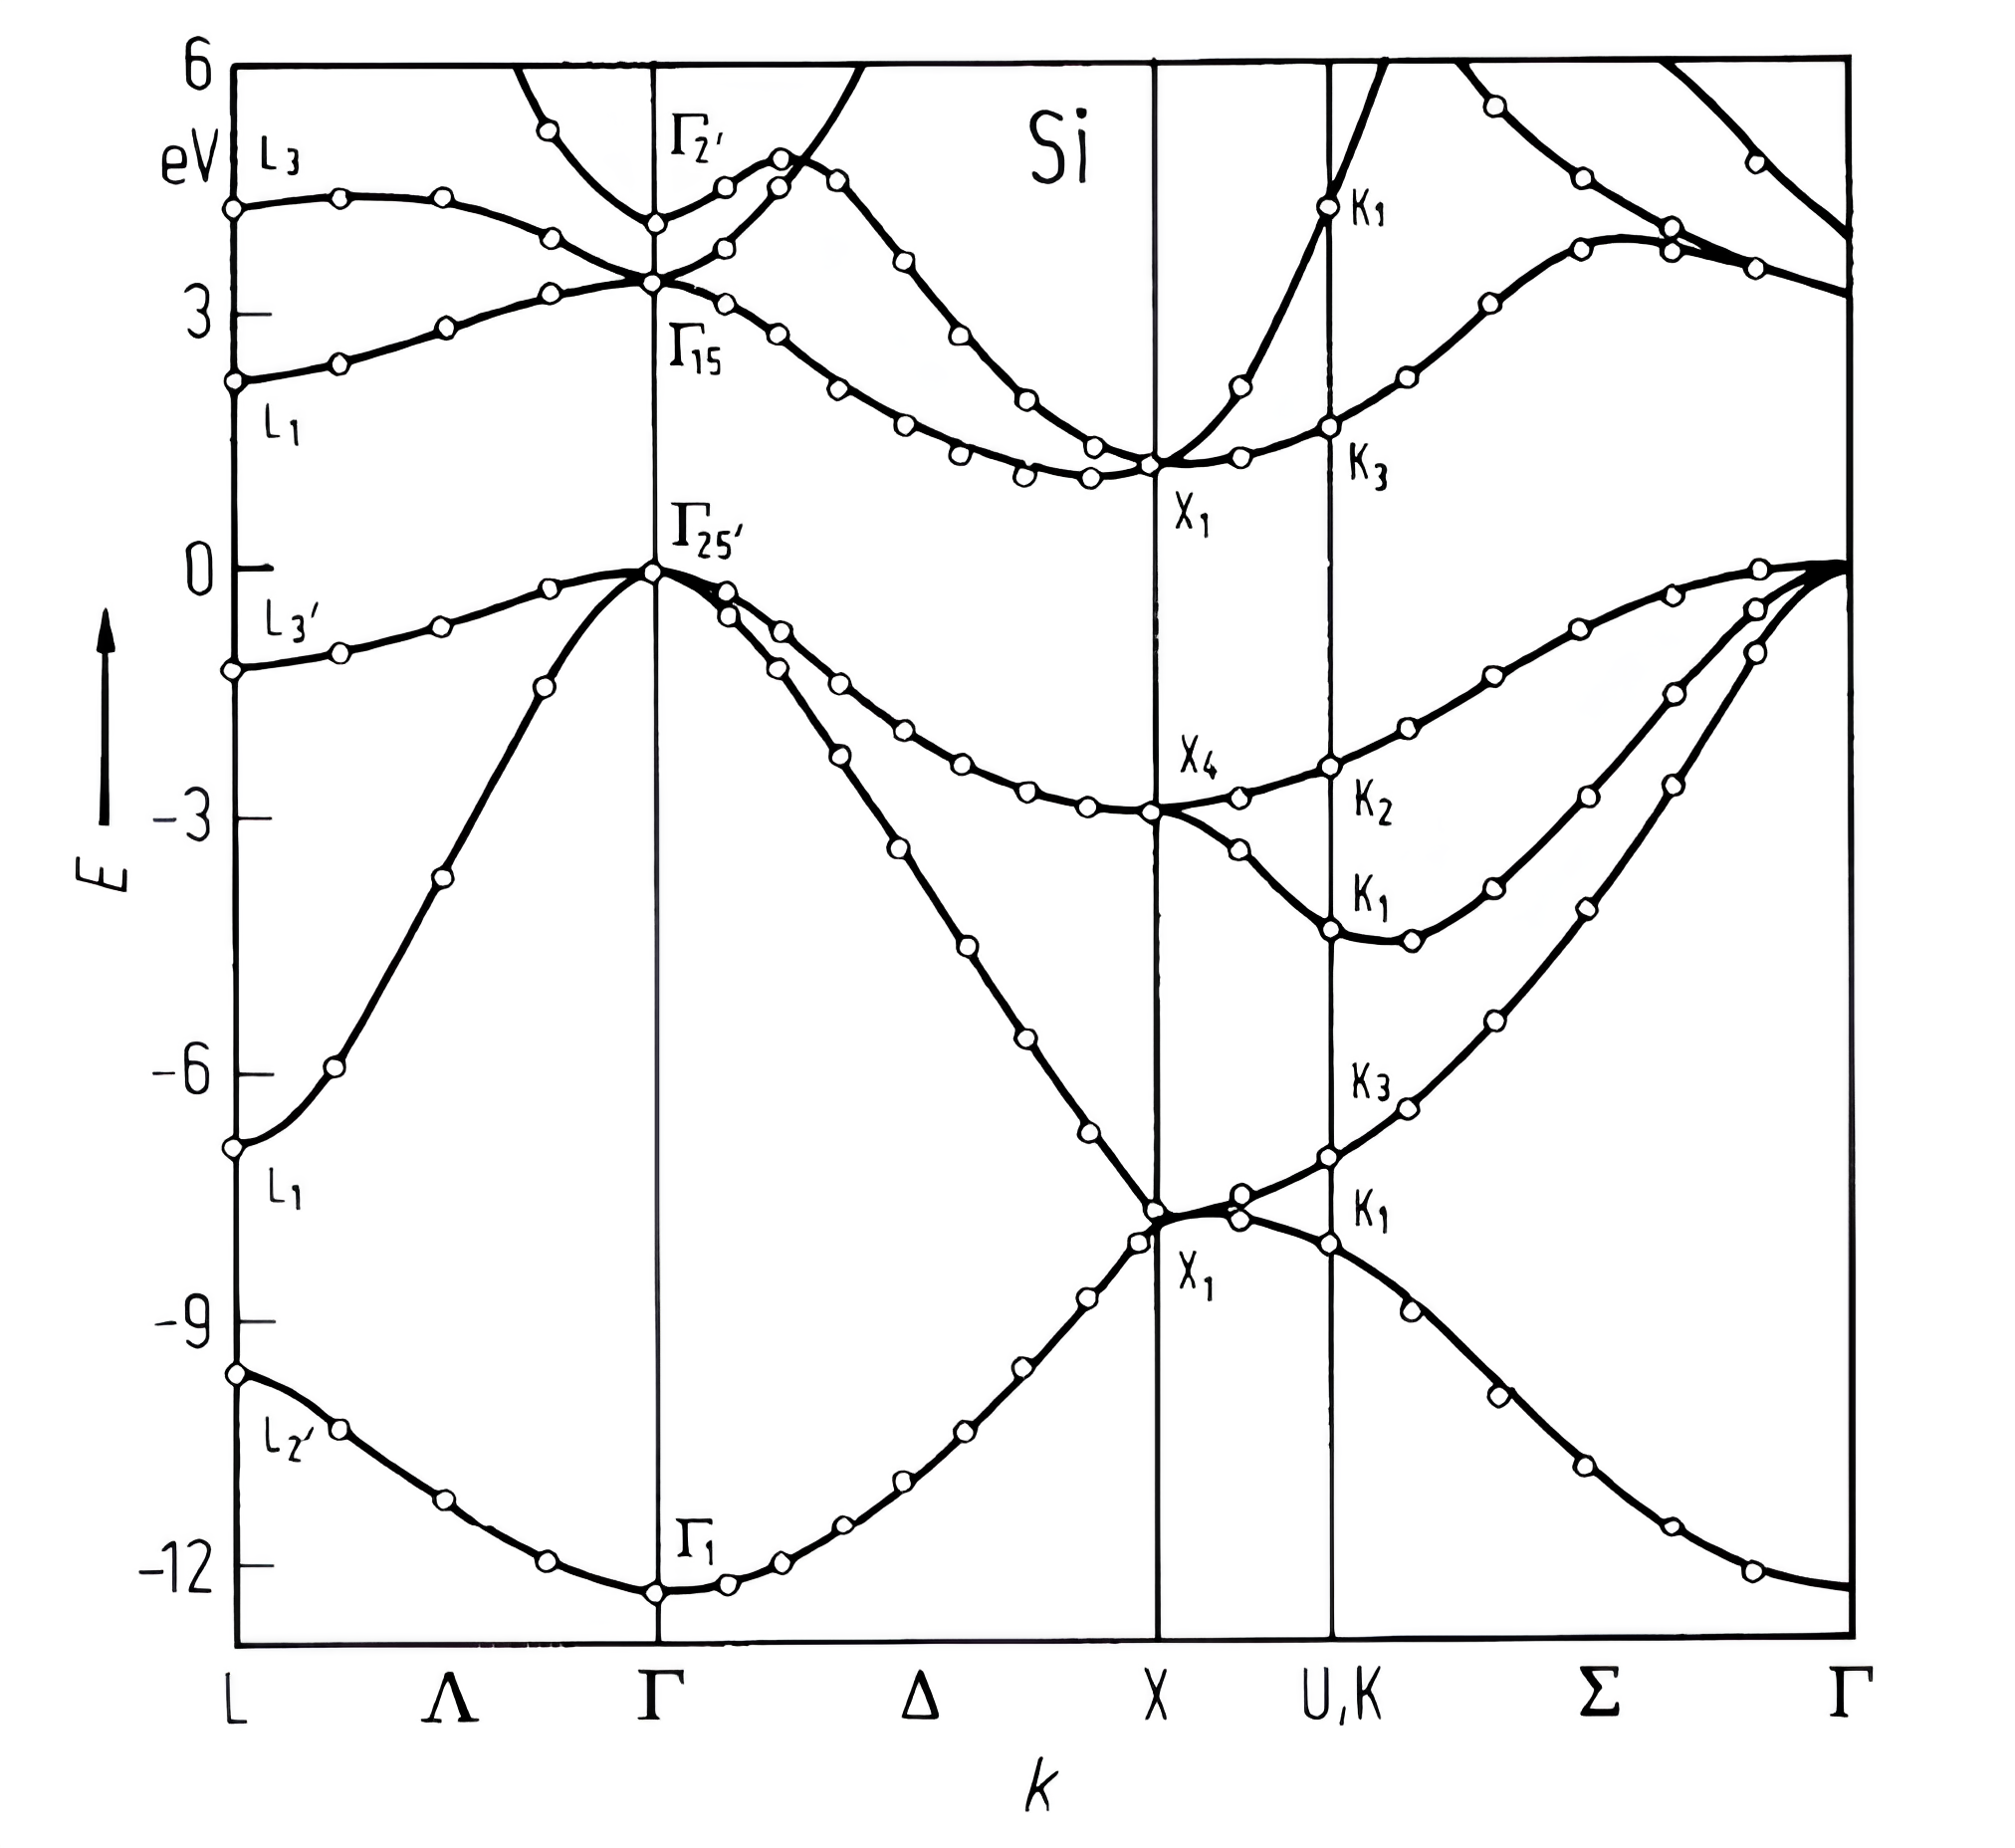
\includegraphics[width=0.6\linewidth]{figures/Si_bandstructure.png}
    \caption{Electronic band structure of crystalline silicon, highlighting the indirect fundamental gap between the valence-band maximum at $\Gamma$ and the conduction-band minima in the $\Delta$ valleys. Taken from \cite{Madelung2002SiBandStructure}.}
    \label{fig:Si_bandstructure}
\end{figure}

\subsection{Electronic Structure near the $\Gamma$ Point}

Despite silicon’s indirect band gap, the $\Gamma$ point ($\mathbf{k}=0$) plays a central role in attosecond spectroscopy. The valence-band maximum resides at $\Gamma$, optical matrix elements are typically strongest near this point, and the symmetry classification of states is most transparent there \cite{Robertson01011983,PhysRev.142.530}. For ultrashort optical excitation, which predominantly induces vertical transitions in $\mathbf{k}$-space, the $\Gamma$-point picture provides a natural starting framework.

At $\Gamma$, the top of the valence band originates from three degenerate $p$-like orbitals ($p_x$, $p_y$, $p_z$) combined with electron spin. Spin–orbit coupling couples orbital angular momentum $L=1$ with spin $S=1/2$, resulting in total angular momentum manifolds with $J=3/2$ and $J=1/2$. The $J=3/2$ states form a fourfold-degenerate manifold at the valence-band maximum, while the $J=1/2$ split-off band lies approximately $44$\,meV below in silicon \cite{Robertson01011983}. 

Within the $J=3/2$ manifold, the states are conventionally labeled as heavy-hole (HH) and light-hole (LH) bands, corresponding to different projections of total angular momentum. Although degenerate at $\Gamma$, these bands differ in curvature: the HH band is flatter and thus associated with a larger effective mass, while the LH band is more dispersive and lighter. For finite $\mathbf{k}$, these bands split and mix, but for the small-$|\mathbf{k}|$ regions relevant to ultrafast optical excitation, the $\Gamma$-point classification remains physically meaningful.

The lowest conduction-band state at $\Gamma$ is predominantly $s$-like and defines the bottom of the direct gap. Although this state lies higher in energy than the $\Delta$-valley minima that define the indirect gap, it plays a crucial role in direct optical transitions and in strong-field excitation scenarios \cite{Robertson01011983}. For sufficiently intense few-cycle pulses, multiphoton and strong-field processes can inject carriers into $\Gamma$-like conduction states even when the photon energy is below the direct gap.

Band-structure calculations show that the conduction-band dispersion near $\Gamma$ is relatively isotropic and approximately parabolic at low energies \cite{PhysRevB.14.556,Benchmarking}. This simplifies the modeling of early-time carrier dynamics in $\mathbf{k}$-space. In the regime considered in this thesis, where few-femtosecond pump pulses induce predominantly vertical excitation, initial carrier injection can be approximated as transitions from HH/LH valence states at $\Gamma$ into conduction states at nearly the same crystal momentum. Subsequent redistribution of carriers into the $\Delta$ valleys occurs on much longer time scales through electron–phonon scattering \cite{Bernardi2014,Marini2013}. 

On attosecond to few-femtosecond time scales, the carrier population therefore remains largely localized in the vicinity of the initial injection region in reciprocal space, making a $\Gamma$-centered description both convenient and physically justified \cite{Schultze2014Si}.




% \subsubsection{Point defects and extended defects in crystalline Si}

% Point defects such as vacancies, interstitials and impurity atoms introduce localized states within the band gap and in the band tails:
% \begin{itemize}
%   \item isolated vacancies generate deep levels in the gap, 
%   \item vacancy clusters and dislocation cores can create a distribution of defect states extending into the mobility gap.\cite{AtomisticBandTailSi,Drabold1999}
% \end{itemize}
% First-principles simulations show that such defect-induced states are strongly localized in real space and can act as trapping centers or recombination sites.\cite{AtomisticBandTailSi,AttaFynn2004}

% From the band-structure point of view:
% \begin{itemize}
%   \item Bloch-like extended states near the valence and conduction band edges coexist with defect-localized states in the gap and tails,
%   \item optical transitions involving defect states lead to additional absorption features below the crystalline band edge and to broadening of the absorption itself.
% \end{itemize}
% In attosecond pump--probe experiments, the presence of such localized states can:
% \begin{itemize}
%   \item modify the initial carrier distribution (e.g.\ by providing sub-gap absorption channels),
%   \item accelerate dephasing of the macroscopic polarization due to spatial inhomogeneity,
%   \item introduce additional, slower components in the transient signal related to trapping and detrapping dynamics.
% \end{itemize}

% \subsubsection{Amorphous silicon: band tails and mobility gap}

% In amorphous silicon (a-Si), long-range translational order is absent, but the local bonding remains predominantly tetrahedral. 
% This has profound consequences for the electronic structure:\cite{Robertson1983,Drabold1999}
% \begin{itemize}
%   \item the concept of a sharp $E(\mathbf k)$ dispersion is replaced by a density of states (DOS) with a \emph{mobility gap},
%   \item the band edges are characterized by exponential band tails of localized states (Urbach tails),
%   \item near the gap, states are spatially localized due to bond-angle and bond-length disorder.
% \end{itemize}

% Atomistic simulations and electronic-structure calculations for large models of a-Si and a-Si:H show that:\cite{Allan1998,DongDrabold1997,AttaFynn2004,Meidanshahi2019,Luo2024}
% \begin{itemize}
%   \item valence-band tails are mainly associated with variations in bond angles and strained bonds,
%   \item conduction-band tails are more sensitive to bond-length disorder,
%   \item dangling bonds (undercoordinated Si atoms) introduce mid-gap states that can dominate transport and recombination,
%   \item hydrogenation (a-Si:H) passivates dangling bonds, reduces mid-gap density of states, and narrows the distribution of tail states.
% \end{itemize}

% Optically, amorphous silicon exhibits:
% \begin{itemize}
%   \item a broadened absorption edge with a characteristic Urbach energy,
%   \item stronger absorption just above the mobility gap compared to crystalline Si because phonon momentum conservation is relaxed by disorder,\cite{Robertson1983,Robertson1983Review}
%   \item substantial inhomogeneous broadening of interband transitions.
% \end{itemize}

% For attosecond spectroscopy, these features imply:
% \begin{itemize}
%   \item the pump predominantly excites carriers into a mixture of extended and localized tail states, rather than into a well-defined $\mathbf k$-point,
%   \item the macroscopic polarization and transient absorption signals dephase more rapidly than in the crystalline case, even in the absence of explicit scattering,
%   \item the concept of $\Gamma$ as a strict crystal-momentum point is no longer applicable, but the \emph{local bonding topology} inherited from crystalline Si still shapes the DOS and selection rules.
% \end{itemize}
% RT-TDDFT in real space is particularly well suited to this situation, since it does not rely on Bloch periodicity and naturally captures band-tail localization and static-disorder-induced dephasing.\cite{Bondi2010,Drabold1999,Dnaya2024,AttaFynn2004}

% \subsubsection{Other physical properties affected by disorder}

% Static disorder and amorphization also influence:
% \begin{itemize}
%   \item \textbf{Effective masses and mobility:} the breakdown of $\mathbf k$ as a good quantum number and the presence of localized states reduce carrier mobility; transport occurs via hopping and percolation through extended regions.\cite{Drabold1999,AttaFynn2004}
%   \item \textbf{Optical constants:} refractive index $n(\omega)$ and extinction coefficient $k(\omega)$ in a-Si differ markedly from crystalline Si, especially near the band edge and in the visible range.\cite{OpticalPropsASi}
%   \item \textbf{Mechanical and vibrational properties:} changes in elastic constants and vibrational density of states modify phonon spectra and thus electron--phonon coupling.\cite{Bondi2010,Zhou2023}
% \end{itemize}

% All of these modifications feed back into attosecond pump--probe observables:
% the broadened DOS and localized tail states affect where carriers are injected and how quickly the macroscopic polarization decays; 
% modified phonon spectra determine the longer-time relaxation pathways; 
% and changes in $n(\omega)$ and $k(\omega)$ influence the propagation and absorption of both pump and probe pulses.

% In summary, silicon as a semiconductor presents a band structure in which the $\Gamma$ point plays a central role for valence-band physics and early-time optical injection, even though the fundamental gap is indirect.
% Static defects and amorphous disorder blur the sharp $\mathbf k$-space picture and generate band tails and localized gap states, which are crucial for interpreting attosecond optical spectroscopy of disordered media.
% RT-TDDFT in real space provides a natural framework to treat both the crystalline reference and its disordered realizations on equal microscopic footing.








\section{Density of States}

The electronic density of states (DOS) provides a fundamental characterization of how structural disorder modifies the electronic structure of silicon. Since ultrafast excitation and transport processes are governed by the available phase space and band dispersion, understanding how disorder reshapes the DOS is essential for interpreting both photoinjection efficiency and subsequent carrier dynamics.

Within RT-TDDFT, the DOS is extracted from the Kohn–Sham eigenvalues obtained for each supercell configuration. While Kohn–Sham eigenvalues do not formally represent quasiparticle energies, they provide a reliable qualitative description of disorder-induced band broadening and gap modification \cite{Onida2002ElectronicExcitations}. 

% We used a $3 \times 3 \times 3$ supercell size in all further calculations both for amorphous and displacement disorder obtaining sufficient convergence, where each primitive cell contains 8 silicon atoms. For each primitive cell we took a grid by coordinate as $18 \times 18 \times 18$ and for k-space $16 \times 16 \times 16$ (where the k-grid decreases proportionally to the size of the supercell along each axis).


All calculations here and in subsequent sections were performed using a $3 \times 3 \times 3$ supercell for both amorphous and displacement disorder, which was sufficient to ensure convergence. Each primitive cell contains eight silicon atoms. We took a real-space grid of $54 \times 54 \times 54$ points and a $5 \times 5 \times 5$ $k$-point mesh which yielded well-converged results.

% For the primitive cell, a real-space grid of $18 \times 18 \times 18$ points and a $16 \times 16 \times 16$ $k$-point mesh were used. For larger supercells, the $k$-point sampling was reduced proportionally along each reciprocal-lattice direction. 

% Consequently, for the $3 \times 3 \times 3$ supercell we used a $5 \times 5 \times 5$ $k$-point grid.



\begin{figure}[h!]
    \centering
    
\includegraphics[width=0.9\linewidth]{all_pdf/dos/pdf/dos_comparison.pdf}
    \caption{Density of states. The degree of displacement disorder is defined by the variance of random atomic displacements in Å, while amorphous disorder is characterized by the SOAP metric. Zero energy is set at the valence band maximum of the crystalline case.}
    \label{fig:dos_total}
\end{figure}

Figure~\ref{fig:dos_total} shows the full valence and conduction bands for crystalline silicon and for increasing disorder. In the crystalline case, sharp van Hove singularities are visible, reflecting well-defined critical points in the band structure. As disorder increases, these features progressively broaden and lose their sharp structure. Such smoothing of van Hove singularities is a generic signature of disorder and has been extensively discussed in the theory of electronic states in non-crystalline materials \cite{MottDavis1979, Sheng2006Localization}.

For displacement disorder, characterized by a root-mean-square atomic displacement in Å, the broadening occurs continuously. In contrast, for amorphous disorder quantified via the SOAP metric, the DOS undergoes more abrupt modifications. This difference reflects the fundamentally distinct structural nature of the two disorder classes: weakly perturbed periodic lattices versus topologically disordered networks.

It is worth noting that small oscillations visible in the crystalline DOS originate from finite $k$-point sampling in the reduced Brillouin zone of the supercell. Increasing $k$-point density reduces these numerical artifacts.

\begin{figure}[h!]
    \centering
    
\includegraphics[width=0.89\linewidth]{all_pdf/dos/pdf/dos_comparison_bandgap.pdf}
    \caption{Density of states near the band gap for displacement and amorphous disorder.}
    \label{fig:dos_gap}
\end{figure}

Figure~\ref{fig:dos_gap} focuses on the region near the band gap. For displacement disorder, the gap decreases gradually as disorder increases. For amorphous disorder, however, the shift of the band edges occurs in a more step-like fashion. This reflects the absence of well-defined Bloch states and the formation of localized states near the mobility edge, a central concept in the theory of amorphous semiconductors \cite{MottDavis1979}.

Band-gap reduction with increasing disorder directly explains the red shift observed in the pump-induced current spectra in the following chapter. Since high-harmonic emission frequencies scale with interband transition energies, disorder-induced gap narrowing shifts spectral weight to lower photon energies.

\begin{figure}[h!]
    \centering
    
\includegraphics[width=0.88\linewidth]{all_pdf/dos/pdf/dos_comparison_bandgap_log.pdf}
    \caption{Logarithmic scale of the density of states near the band edge highlighting exponential tail formation.}
    \label{fig:dos_log}
\end{figure}

In Figure~\ref{fig:dos_log}, the DOS is plotted on a logarithmic scale to analyze the band-edge tails. In disordered semiconductors, the DOS near the band edge often follows the Urbach law,
\[
g(E) \propto \exp\left(\frac{E - E_0}{E_U}\right),
\]
where $E_U$ is the Urbach energy \cite{Urbach1953}. The Urbach tail describes exponential decay of the DOS into the gap due to disorder-induced fluctuations of the potential landscape.

Although a clean exponential region is difficult to isolate in our finite supercells, the average slope of $\ln g(E)$ near the valence band edge decreases with disorder. This trend qualitatively correlates with the transport and dephasing times extracted later in this work. Physically, larger Urbach energies correspond to stronger spatial fluctuations of the local potential and therefore enhanced scattering.

From a localization perspective, exponential tails arise from spatially localized states in fluctuating potentials \cite{Sheng2006Localization}. Such states contribute to enhanced inhomogeneous broadening and accelerate free-induction decay of coherent dipole oscillations.

Overall, the DOS analysis reveals three central disorder effects:
First, progressive smoothing of van Hove singularities and reduction of band dispersion.
Second, systematic band-gap narrowing and red shift of transition energies.
Third, formation of exponential band-edge tails associated with disorder-induced localization.

These modifications of the electronic structure form the microscopic basis for the disorder dependence of photoinjection, current dynamics, and coherent oscillations discussed in subsequent chapters.


\begin{figure}[h!]
    \centering
    
\includegraphics[width=0.9\linewidth]{all_pdf/lr/pdf/im_epsilon.pdf}
    \caption{Imaginary part of the dielectric function.}
    \label{fig:epsilon_im}
\end{figure}


Figure~\ref{fig:epsilon_im} shows the imaginary part of the complex dielectric function, $\varepsilon_2(\omega)$, which is directly associated with optical absorption and interband transitions. For the displacement disorder case, the direct band gap decreases systematically from 2.52 eV in the ideal crystal to 2.13 eV, 1.48 eV, 1.00 eV, and 0.60 eV as the displacement amplitude increases up to 0.1 Å. Beyond this point, the reduction becomes limited by the finite width of the time window used to compute the linear response, which in our case is 60 fs. In crystalline silicon, the absorption onset is sharp and reflects the well-defined band gap and van Hove singularities of the ordered band structure. 

With increasing disorder, two systematic effects are observed. First, the absorption edge shifts to lower photon energies, indicating band-gap narrowing. This red shift directly mirrors the reduction of the gap seen in the density-of-states analysis (Fig.~\ref{fig:dos_gap}). Second, the absorption spectrum becomes progressively broadened and smoother. The sharp structures present in the crystalline case are washed out as disorder increases, consistent with the smoothing of van Hove singularities observed in the DOS (Fig.~\ref{fig:dos_total}). 

Physically, the broadening of $\varepsilon_2(\omega)$ reflects the increasing distribution of transition energies due to local potential fluctuations and reduced translational symmetry. The formation of band-tail states near the mobility edge, visible in the logarithmic DOS (Fig.~\ref{fig:dos_log}), contributes to a gradual rather than abrupt onset of absorption. As a result, the energy at which absorption begins decreases with disorder, and the edge becomes less sharply defined. 

Thus, the modifications of the imaginary part of the dielectric function provide an optical manifestation of the electronic-structure changes induced by disorder, linking band-gap reduction and DOS broadening directly to measurable absorption spectra.



\section{Applicability of Strong Effective Disorder and Large Band-Gap Renormalization}
\label{sec:applicability_effective_disorder}

In our RT-TDDFT supercell calculations, increasing structural disorder can reduce the Kohn--Sham band gap by up to $\sim 1$~eV and even less to the point of disappearance, and produces pronounced broadening of the band-edge DOS and broadened absorption spectrum. At first sight, such large gap changes may appear inconsistent with experimentally realized amorphous silicon, where change in band gap is typically around 0.1 eV. This motivates a clarification of what the disorder parameter in the present work is meant to represent.

The central point is that the goal of this thesis is not to reproduce the long-time, equilibrium electronic gap of amorphous silicon. Rather, the disorder parameter is used as an \emph{effective ultrafast scattering knob} that controls (i) the spectral width of interband transition energies contributing to macroscopic polarization and current, and (ii) the rate of elastic momentum randomization within the short ($\lesssim 30$~fs) time window relevant for attosecond pump--probe observables.
In this regime, measured signals are primarily sensitive to coherence loss and transport relaxation rather than to the equilibrium definition of the optical gap. A clear example is provided by attosecond transient-absorption in crystalline Si: the electronic response to carrier injection builds up on sub-femtosecond time scales, while lattice-driven band-gap modifications appear only later, on $\sim 60\pm 10$~fs time scales associated with the fastest optical phonon \cite{Schultze2014Si}. This separation of time scales justifies focusing on ultrafast electronic decoherence mechanisms when comparing to attosecond-scale measurements.

Homogeneous dephasing of an interband coherence $p_{\mathbf{k}}(t)$ is commonly modeled as
\begin{equation}
p_{\mathbf{k}}(t)\propto e^{-i\omega_{cv}(\mathbf{k})t}\,e^{-t/T_2},
\end{equation}
which corresponds in frequency space to a Lorentzian broadening of optical transitions with a characteristic width
\begin{equation}
\Gamma \sim \frac{\hbar}{T_2}.
\label{eq:Gamma_T2_applicability}
\end{equation}
Therefore, the femtosecond dephasing times frequently inferred in ultrafast solid-state spectroscopy correspond to very large effective broadenings. For example, $T_2=10$~fs implies $\Gamma\simeq 0.066$~eV, while $T_2=2$~fs implies $\Gamma\simeq 0.33$~eV, and $T_2=1$~fs implies $\Gamma\simeq 0.66$~eV. Broadening on the scale of $0.1$--$1$~eV is thus the natural spectral signature of coherence decay in the experimentally relevant $1$--$10$~fs range.

Ultrashort dephasing times of this order are not an artifact of our modeling: they are widely used and, in several settings, directly supported by experiments.
In solid-state high-harmonic generation (HHG), reciprocal-space semiconductor-Bloch-equation simulations often require phenomenological dephasing times of only a few femtoseconds to reproduce measured spectra. Recent work has explicitly analyzed the \emph{origin} of these ``extremely short dephasing times'' and argues that they are required to suppress contributions from large electron--hole separations during recombination \cite{PhysRevResearch.6.043005}. Complementarily, phenomenological decoherence terms (e.g.\ imaginary potentials) have been introduced and validated against HHG trends, underscoring that femtosecond-scale dephasing is a key control parameter in solid HHG modeling \cite{PhysRevA.103.063109}.
Moreover, HHG-based metrology can access dephasing times directly: recent experiments used high-harmonic polarimetry to extract an electron--hole dephasing time $T_2$ of a few femtoseconds \cite{Heide:22}. Although performed in a different material class, this result demonstrates that HHG observables can indeed be governed by femtosecond-scale coherence loss.
Finally, even within silicon-specific ultrafast spectroscopy, phase-resolved transient absorption with sub-5-fs excitation reports an ultrafast single-electron momentum relaxation time of $\sim 10$~fs and Drude collision times down to a few femtoseconds at the earliest delays, together with a time-dependent optical effective mass \cite{Worle2021}. This directly supports the physical relevance of the dephasing/transport window explored in the present simulations.

Within this perspective, the large reduction of the bandgap observed in our disordered supercells should be interpreted as a convenient proxy for accessing the regime of large effective broadening $\Gamma$ and rapid dephasing (Eq.~\ref{eq:Gamma_T2_applicability}). In strongly disordered configurations, the notion of a single sharp Bloch band edge is replaced by broadened band-edge manifolds with tail states; consequently, optical transition energies relevant for current and polarization become distributed over a wide range.

We therefore view the disorder parameter primarily as an \emph{effective ultrafast decoherence parameter} rather than a literal representation of equilibrium amorphous-silicon band-gap renormalization. This approach is appropriate for the thesis focus: linking disorder-induced DOS broadening, pump photoinjection, intraband current relaxation, and coherent-current-oscillation dephasing within a $0$--$30$~fs window. At the same time, quantitative comparison to equilibrium optical gaps of a-Si:H would require realistic amorphous structural models (including hydrogen, defect statistics, and larger supercells) and, ultimately, quasiparticle corrections beyond Kohn--Sham eigenvalues \cite{Onida2002ElectronicExcitations}. Those extensions lie outside the present scope.